\newpage\section{Design and Development of the Artefacts}

The artifact, which is intended to improve experimental research in behavioral data analytics, is to be implemented as a software component or application. In this step, a suitable architecture is developed based on the established requirements. For this purpose, the application is first fundamentally conceptualized. This involves analyzing possible technologies and the corresponding processes. The architecture is then implemented in practice on the basis of this basic concept.

\subsection{Process Conceptualization}

%This section focuses on the basic design of the application. For this purpose, the processes based on the requirements are presented first, which must be implemented by the application. Subsequently, technologies are presented which are used for their implementation.

%\subsubsection{Process Mechanisms}

In order to effectively implement the requirements for the application, the processes described by the requirements and validated by the test cases are represented in the following by swim lane diagrams. The goal of this is to illustrate the individual processes in a technology-independent manner. The reason for this is that the individual processes are initially presented in generalized form, irrespective of technological restrictions or limitations. The following Swim Lane diagrams represent the individual steps of the experiment. Swim lane diagrams depict processes by showing business activities in relation to each other and how they are associated with each other (\cite{Caudle.2009}).A large part of the final functionalities can be divided into two different categories. An example of this are the requirements (F2, F3 and N5.1), whereby the application should offer both the possibility to read in and save user data and to make the experiment setup reusable. These requirements can be summarized in functions and data concerning the experiment and functions and data concerning the participants. The two lanes \enquote{Participant file} and \enquote{Experiment file} are representative for those two categories and data sources. The \enquote{User} lane shows the activities performed by the test subjects, the \enquote{Experimental file} lane shows all activities that can be associated with the experimental set-up, and the \enquote{Patricipant} file lane shows all activities that are related to the data or distribution of the test subjects. 

\begin{figure}[htbp]
    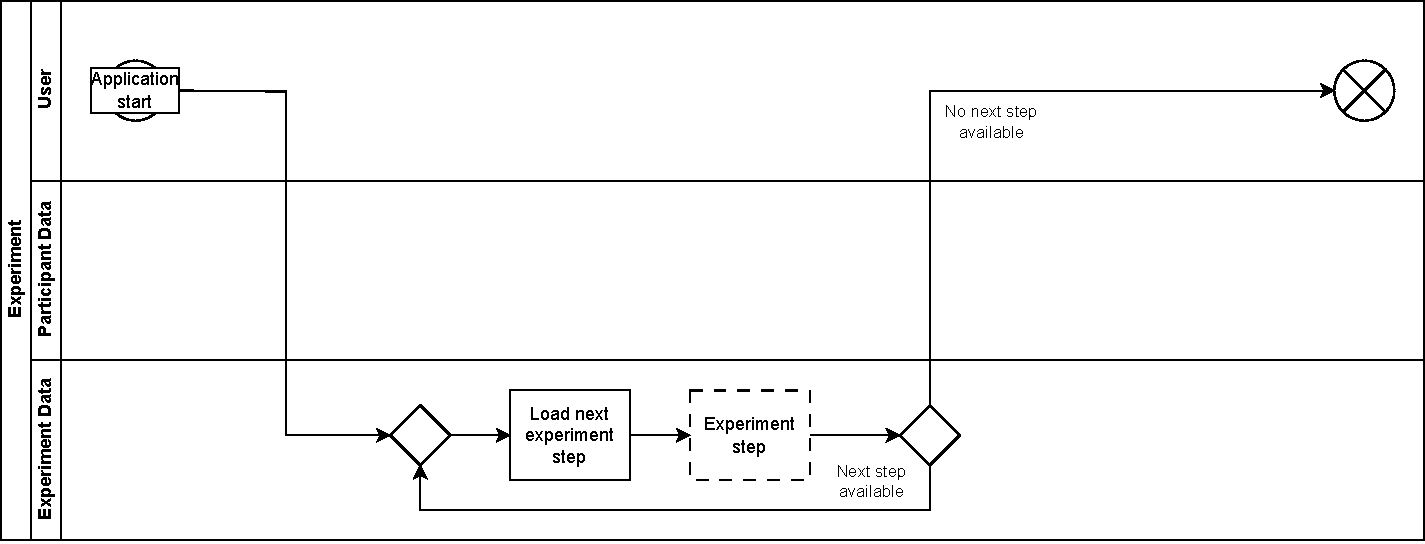
\includegraphics[width=0.99\textwidth, keepaspectratio]{content/05_design_and_dev_artefacts/ExperimentSwimLane.drawio.pdf}
    \caption{Experiment - Swim lane}    
    \label{fig:experimentSwimLane}
\end{figure}

Figure \ref{fig:experimentSwimLane} shows the basic structure of an experiment with the conceptualized application. The whole experiment is divided into different experiment steps, which are executed one after the other until the experiment is completed. The application is started first and then the first step of the experiment is executed. This could be for example an information message for the participants. After that the next step is executed if another step is available. If no further step is available, the experiment ends. This simple abstraction of an experiment concentrates on the essentials and thus allows the most flexible and adaptable construction kit for an experiment. The individual steps of the experiment, which are executed one after the other, can be customized by the person performing the experiment as well as mapped by standard steps. The standard steps represent steps which have to be used in a multitude of experiments and thus partially represent requirements. In the following, some of these experiment steps which illustrate standard steps that are included in the application are illustrated with the help of swim lane diagrams. Figure \ref{fig:DataInputSwimLane}, \ref{fig:groupAllocationSwimLane}, \ref{fig:questionairSwimLane} and \ref{fig:infoScreenSwimLane} represent these standard steps. The dashed box \enquote{Experimental Step} of figur \ref{fig:experimentSwimLane} can be replaced by any number of these. For this reason, the graphics mentioned also begin and end in the \enquote{Experimental file} lane.

\begin{figure}[htbp]
    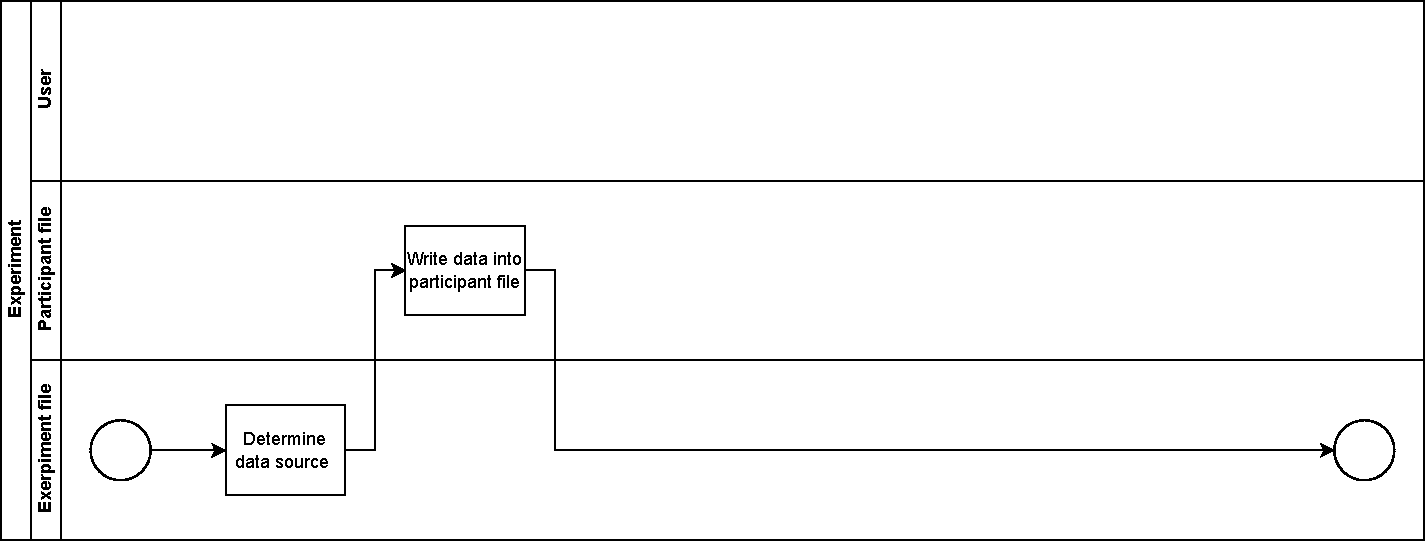
\includegraphics[width=0.99\textwidth, keepaspectratio]{content/05_design_and_dev_artefacts/DataInputSwimLane.drawio.pdf}
    \caption{Data input step - Swim lane}    
    \label{fig:DataInputSwimLane}
\end{figure}

Figure \ref{fig:DataInputSwimLane} represents the process step of reading data from one or more sources. The assumption is that this data must first be processed or standardized before it can be meaningfully assigned to the participants.

\begin{figure}[htbp]
    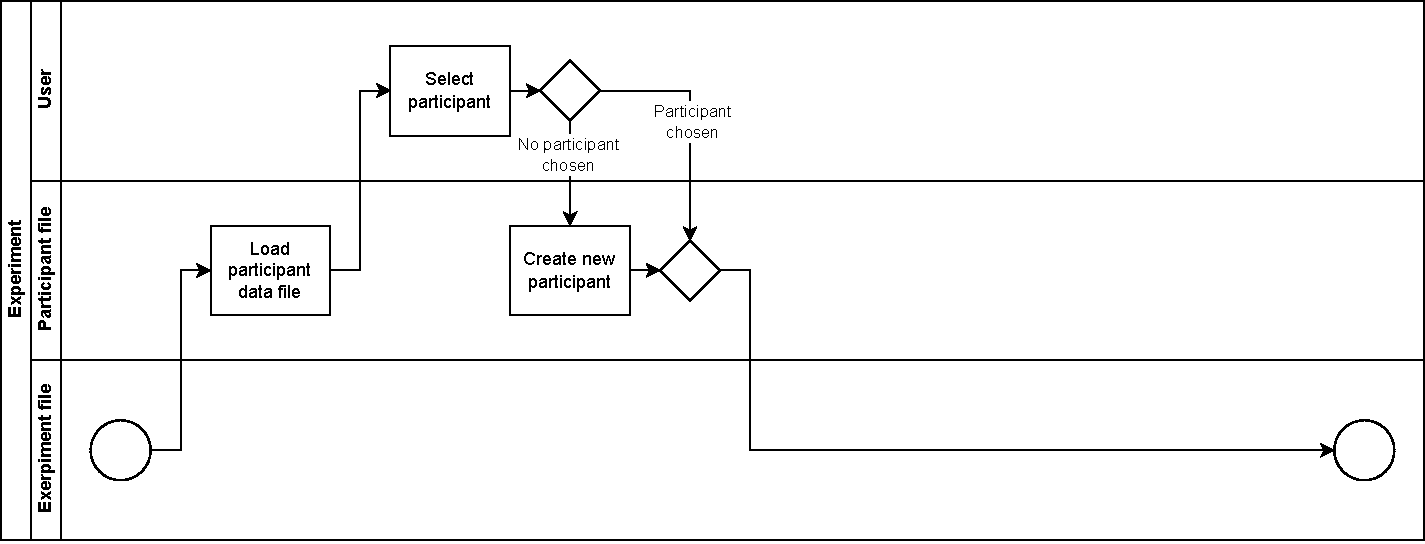
\includegraphics[width=0.99\textwidth, keepaspectratio]{content/05_design_and_dev_artefacts/ChooseTestSubjectSwimLane.drawio.pdf}
    \caption{Choose test subject step - Swim lane}    
    \label{fig:ChooseTestSubjectSwimLane}
\end{figure}

Figure \ref{fig:ChooseTestSubjectSwimLane} enables the mapping between the test subject and their ID which will be used for the rest of the experiment.

\begin{figure}[htbp]
    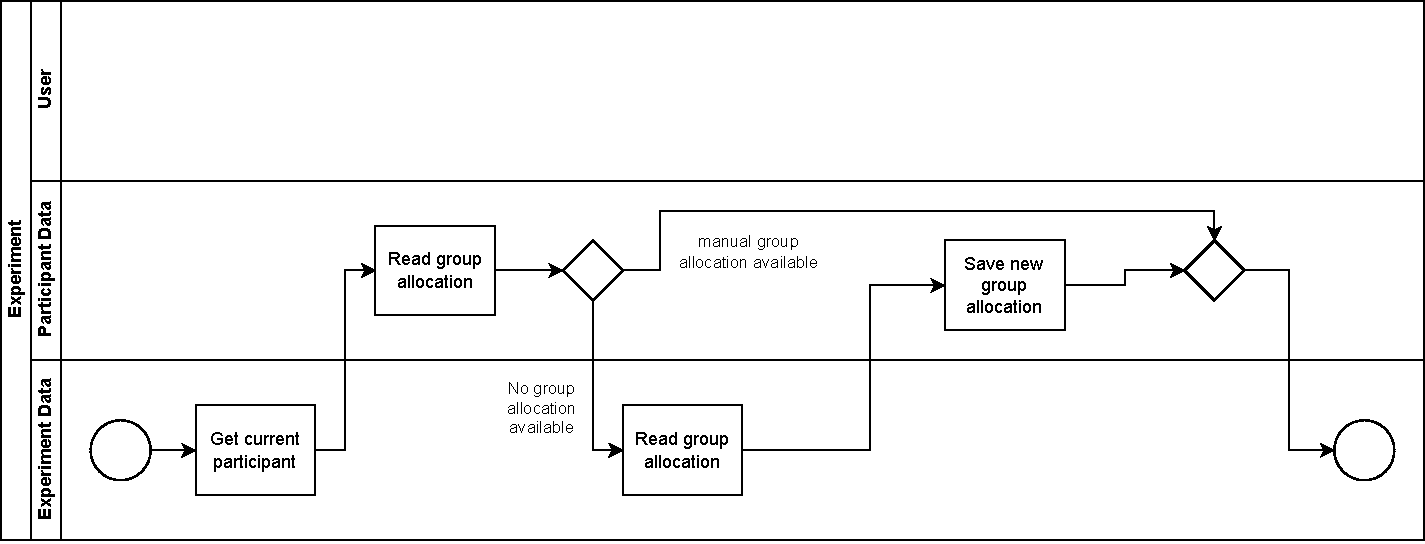
\includegraphics[width=0.99\textwidth, keepaspectratio]{content/05_design_and_dev_artefacts/GroupAllocationSwimLane.drawio.pdf}
    \caption{Group allocation step - Swim lane}    
    \label{fig:groupAllocationSwimLane}
\end{figure}

Figure \ref{fig:groupAllocationSwimLane} represents the process of assigning individual participants into groups. This can either be the case that participants are divided according to a predefined group, arbitrarily or according to certain criteria.

\begin{figure}[htbp]
    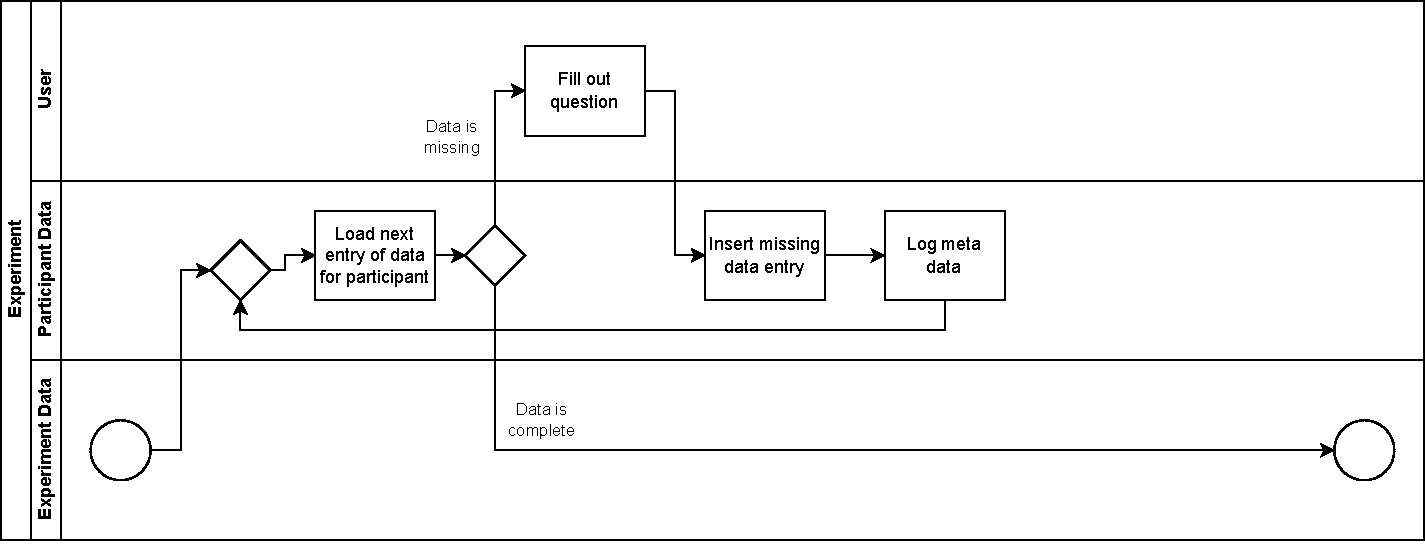
\includegraphics[width=0.99\textwidth, keepaspectratio]{content/05_design_and_dev_artefacts/QuestionairSwimLane.drawio.pdf}
    \caption{Questionair step - Swim lane}    
    \label{fig:questionairSwimLane}
\end{figure}

Figure \ref{fig:questionairSwimLane} is used to complete the data of the participants. For this purpose, test subject questions are asked based on missing data which are to be answered by the participant. An example would be a test subject for which the age is missing. An input field is automatically displayed for the participant to fill in the missing data. If all data for a test subject is available, nothing is displayed.

\begin{figure}[htbp]
    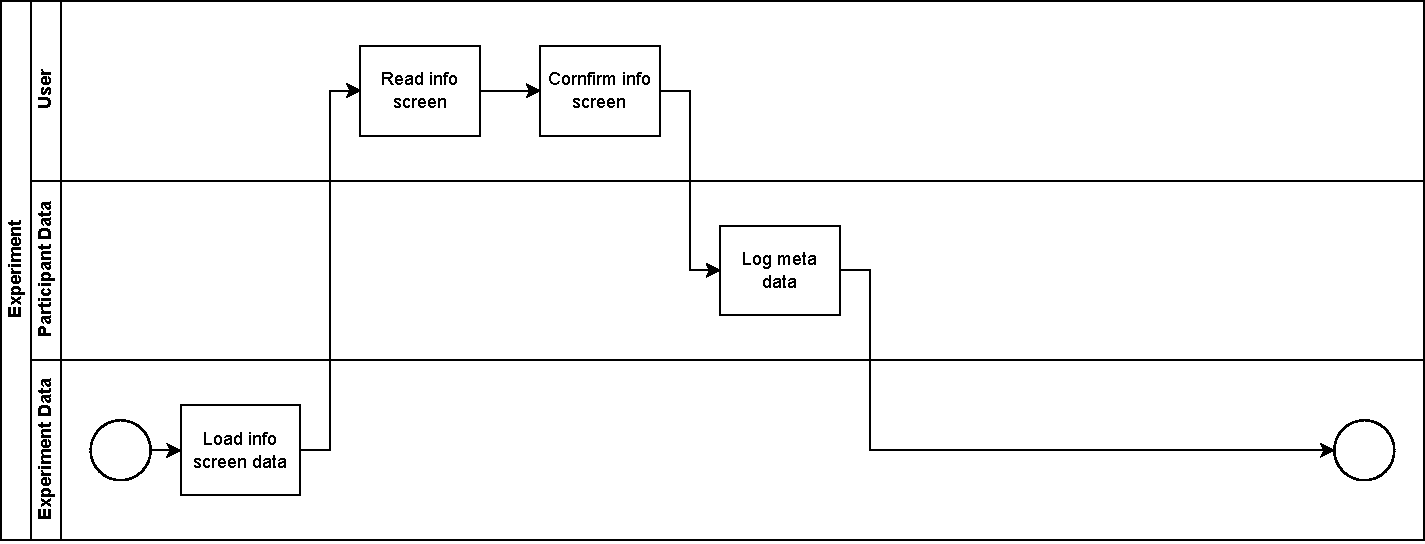
\includegraphics[width=0.99\textwidth, keepaspectratio]{content/05_design_and_dev_artefacts/InfoScreenSwimLane.drawio.pdf}
    \caption{Info screen step - Swim lane}    
    \label{fig:infoScreenSwimLane}
\end{figure}

Figure \ref{fig:infoScreenSwimLane} displays information to the Test Subjects and can be used both as a means of notification during an experiment and as a representation of information.

\subsection{Technology Selection}

In order to select appropriate technologies for the implementation of the application, the established requirements must be considered. It can be assumed that all functional requirements can be implemented by any modern programming language that is turing complete. The non-functional requirements N3.1 (Evaluation of Data), N3.2 (Vizualize Final Data), N7.1 (Multi-Source) are represented by the availability of various interfaces. Furthermore, the two non-functional requirements N1.2 (Time-Flexibility) and N6.1 (Monitoring of Study) are left out as these refer to the way the application is implemented and not its technological nature. This leaves requirements N1.1 (Distand Communication),  N4.1 (Simplicity), N5.1 (Reusable), N5.2 (Interoperability), N5.3 (Openness of Platform), N8.1 (Advanced User Interface) and the afformentioned availability of interfaces for selecting a suitable technology. In the following chapters, various technologies and tools are presented that are intended to meet these requirements.

%interfaces
%Distand Communication
%Simplicity
%Reusable
%Interoperability
%Openness of Platform
%Advanced User Interface


\subsubsection{Android and Android Studio}

Android is an open source operating system for mobile devices which was first announced by Google in 2013. To date, Android has achieved a market share of over 90\% in the mobile sector and is the most used operating system over all, being used in almost every second device (\cite{statcounter.2023}, \cite{Richter.2019}). The standard development environment to develop Android is the \ac{ide} Android Studio, which supports a wide range of developer tools and functionalities. As an open source project and, due to its high distribution on various devices Android suits the openness of platform and interoperability requirement (\cite{Richter.2019}). Applications for the Android operating system are called apps. These apps are programs designed for touch inputs, which are specifically designed for mobile devices. However, as a widely used open source operating system, Android also supports other input options, advanced network capabilities and a variety of interfaces and extensions. Thus it can be assumed that the interface and distand communication requirements can be fulfilled through the usage of Android (\cite{Richter.2019}). The two programming languages that can be used to develop Android apps are Java and Kotlin. These apps then can be tested either directly on an Android device or on a variety of virtual devices integrated in Android Studio, which further facilitates the development of said applications (\cite{Richter.2019}). As a mobile operating system, one of Android's main focuses is the user interface as an input function, in addition to network functionalities and a variety of interfaces. Android therefore has a wide range of design guidelines, interface functionalities and is updated at very regular intervals (\cite{statista.2023}). Due to these regular updates, the widespread use of Android and the focus on \ac{ui} intensive use cases, it can be assumed that an app developed in Android supports the latest user interface technologies and therefore fulfills the advanced user interface.


\subsubsection{Java}

Java is a programming language originally developed by Microsystems. Since 2009 Java is part of the product portfolio of Oracle Corporation. Java is an object-oriented programming language, which makes it an universally applicable and robust programming language (\cite{Ullenboom.2017}). Unlike many other programming languages, one of the special features of Java is its platform independence. Most programming languages use a compiler or interpreter to translate program code into byte code, which varies depending on the hardware and can only be executed on the appropriate processors. Java avoids this limitation by first having a compiler translate the Java program code into byte code, which is then executed via an interpreter in a virtual environment which is called \ac{jvm}. In this way, Java code can theoretically be executed on any system (\cite{Ullenboom.2017}). This makes Java not only a programming language but also a runtime system, which is made clear by the naming of the Java Platform by Oracle. The Java Platform supports beside Java itself also the execution of some other programming languages as for example Kotlin (\cite{kotlinlang.2023}), which become more and more popular. Due to this fact, Java is especially suitable for the implementation of the application Based on the requirements N5.1 (Reusable) and N5.2 (Interoperability). Java also supports a variety of programming concepts through standard libraries. These include data structures, string processing, date/time processing, graphical interfaces, input/output, network operations, threads and more (\cite{Ullenboom.2017}), which ensures the N1.1 (Distand Communication) requirement and the availability of interfaces. The Java runtime environment also enables fast code execution and comes with various utilities such as a garbage collector and output name handlers. The syntax of Java is generally considered to be very easy to understand and beginner-friendly (\cite{Ullenboom.2017}), fulfilling the requirement N4.1 (Simplicity). In addition to technical aspects, Java is also Open-Source, extremely widespread, popular and in a variety of literature available (\cite{Ullenboom.2017}), which generally indicates the openness of platform of the Java Platform (Requirement N5.3 Openness of Platform). Disadvantages of Java, which are also mentioned for the sake of completeness, mainly relate to very specific platform-dependent use cases. Since Java was developed as a general-purpose programming language and platform-independent, it is very difficult to access hardware or drivers directly. However, these use cases are irrelevant in the course of this work (\cite{Ullenboom.2017}). 


\subsection{System Architecture}

Overall, it can be summarized that the non-functional requirements, which consider properties of the system, are completely fulfilled by using the Android operating system in combination with the Java programming language.In general, most of the requirements could already be met by both Android and Java alone, so the combination of the two provides a solid foundation for meeting the remaining requirements. For this reason, the artifact is implemented in the form of a mobile Android application.

For the sake of completeness, it should be noted at this point that the conceptualized architecture and process flows could also be implemented with the help of other technologies. Furthermore, there is the possibility that at a later point in time another technology combination may be able to better reflect the requirements. At this point in time, however, the requirements can best be met by the combination of Android and Java. In addition, for the reasons mentioned, it can be assumed that this combination of technologies will remain the best way to implement the requirements in the long term. However, the fact that these technologies will no longer be up to date at a later point in time exists, but cannot be ruled out for any technology. On the contrary, Android and Java are a sensible and sustainable choice in the long term for the above-mentioned reasons according to the current state of research.


Android Developer Doku (\cite{Google.2023})

Customizing ist blöd (\cite{Chou.2008})



\subsubsection{Activitys}

\begin{figure}[htbp]
    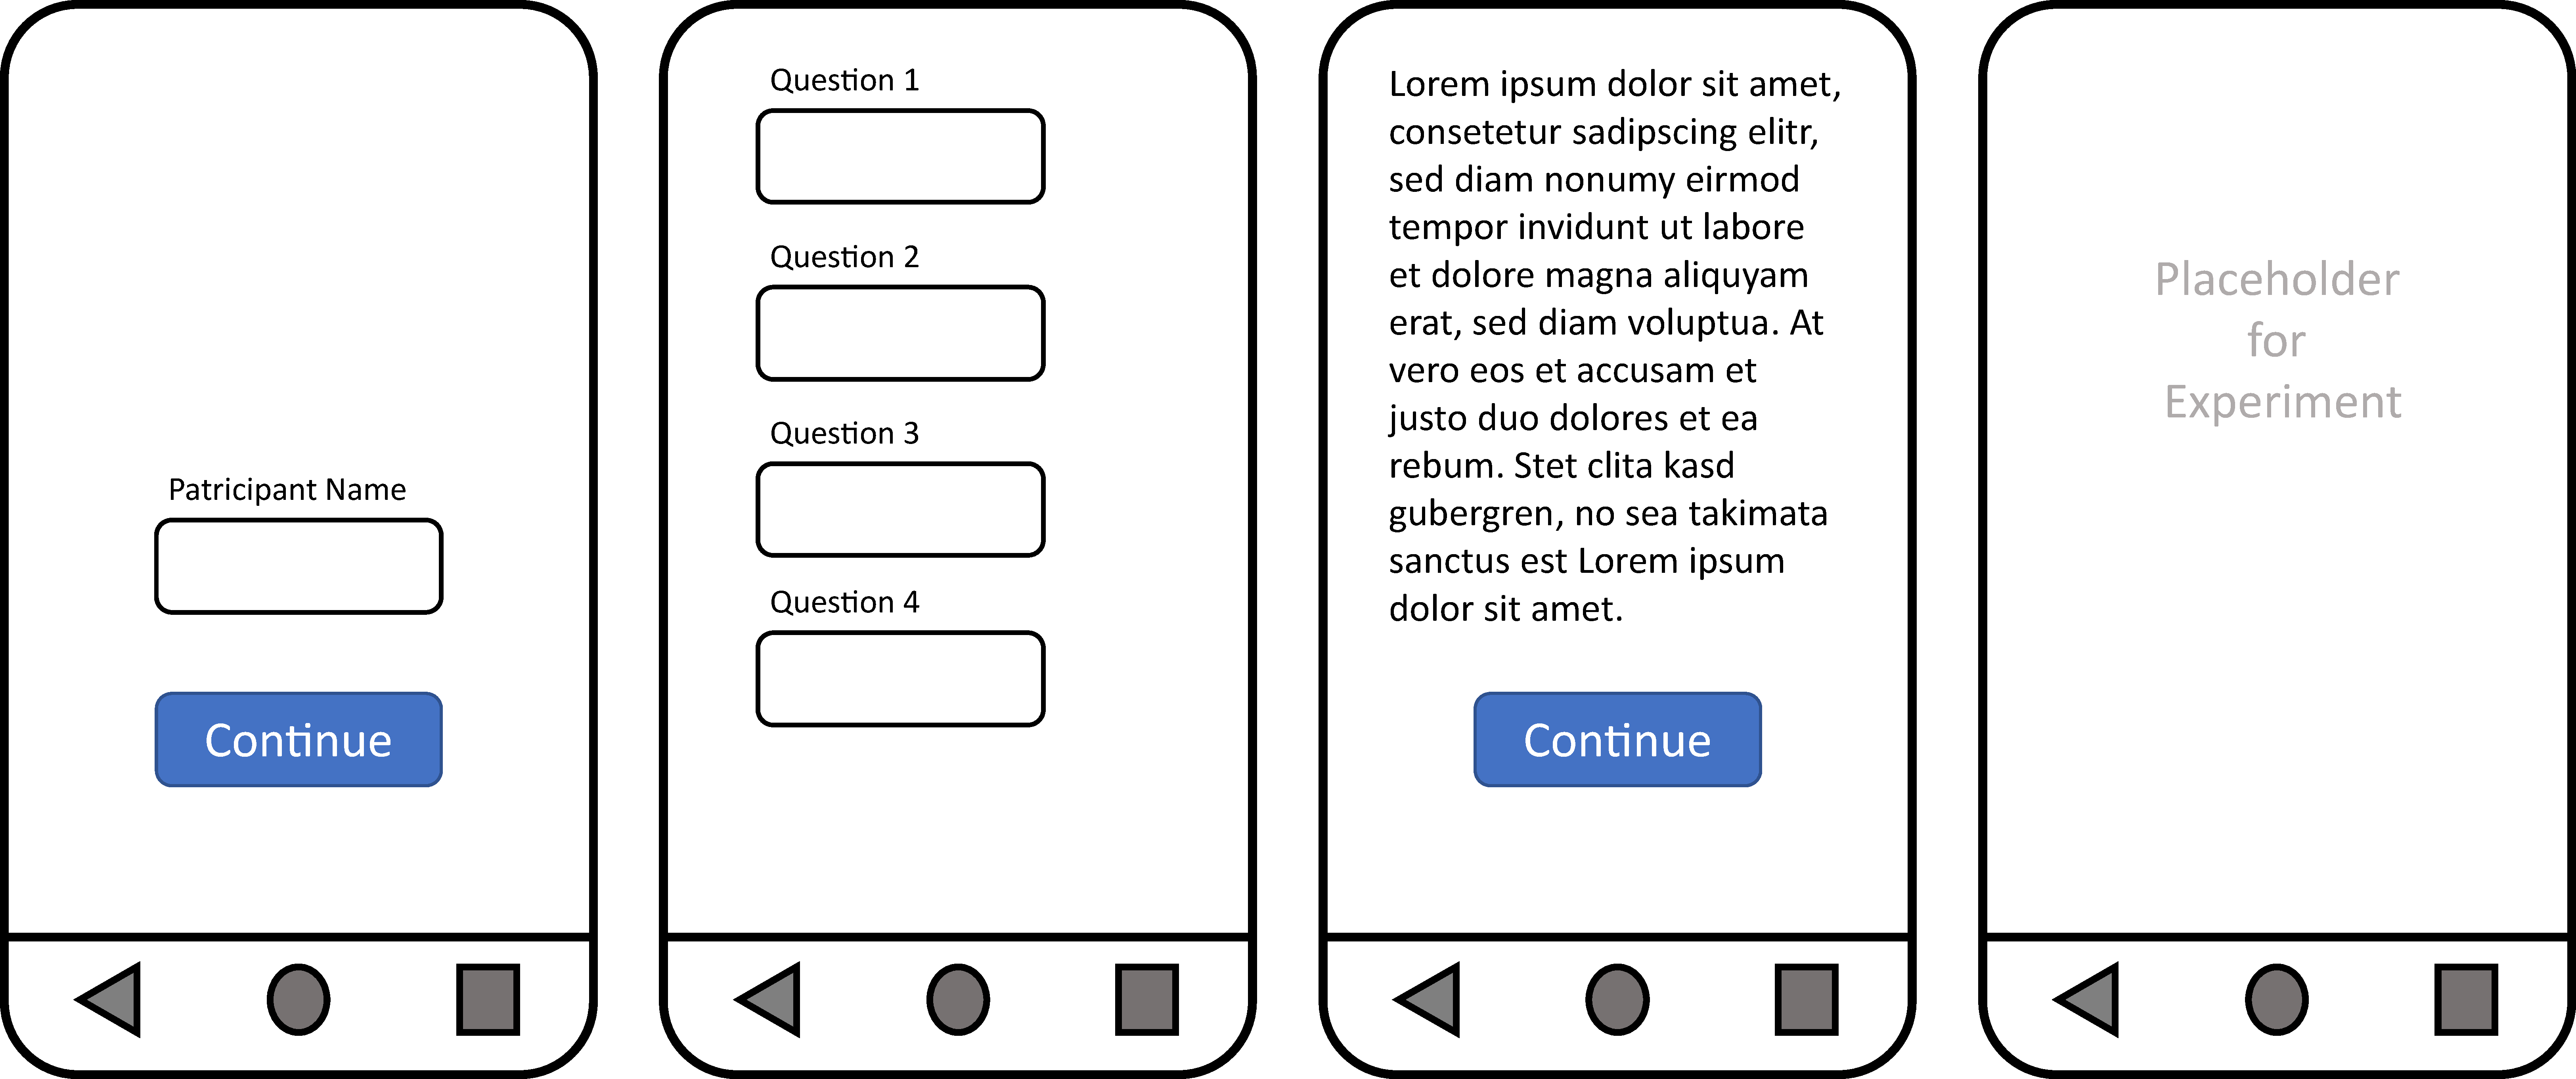
\includegraphics[width=0.99\textwidth, keepaspectratio]{content/05_design_and_dev_artefacts/Activities.pdf}
    \caption{Adroid Studio Activitys}    
    \label{fig:activitiesMockUp}
\end{figure}


\subsubsection{Customizing and System Output}

This section is intended to provide an overview of the technological framework used and the basic architecture of the application. This section focuses primarily on a basic overview, while the next sections go into more detail about the individual components.




%\subsection{Prototype Development}
